% fig/fig.tex
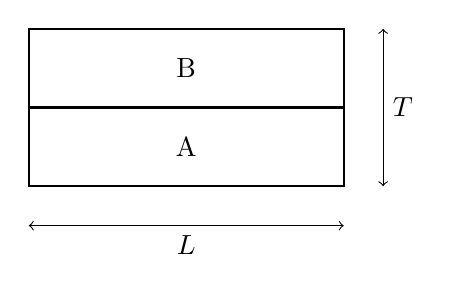
\begin{tikzpicture}
% Rectangle with region labels A and B
\draw[thick] (0,0) rectangle (4,2);
\draw[thick] (0,1) -- (4,1); % Middle line separating A and B
\node at (2,0.5) {A};
\node at (2,1.5) {B};

% Labeled dimensions
\draw[<->] (0,-0.5) -- (4,-0.5) node[midway, below] {$L$};
\draw[<->] (4.5,0) -- (4.5,2) node[midway, right] {$T$};

\end{tikzpicture}
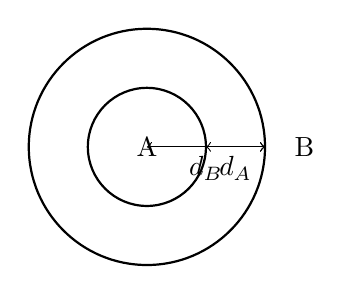
\begin{tikzpicture}
\draw[thick] (0,0) circle (1.5); 
\draw[thick] (0,0) circle (0.75); 
\node at (0,0) {A}; 
\node at (2,0) {B}; 
\draw[<->] (1.5,0) -- (0.75,0) node[midway, below] {$d_A$};
\draw[<->] (0,0) -- (1.5,0) node[midway, below] {$d_B$};
\end{tikzpicture}

